%%%
%%% Grafiken
%%%

%%%
%%% Autor: Export von Grafiken B. Hartmann.
%%%

\part{Graphics}
\begin{frame}
\thispagestyle{empty}
\textbf{\huge{Graphics}}
\end{frame}

\begin{frame}{Graphics Contents}
 \tableofcontents
\end{frame}


\section{Preface}
\begin{frame}{Graphics}
% \begin{minipage}{11cm}
 The next slides will provide an example of different types of graphics. Detailed examples and syntax for modification of graphic title, titles for the axis or combination of multiple graphics see \textcite[Chap. 6]{Kohler12en} and in-depth with lots of images \textcite{Mitchell2012}.
% \end{minipage}
\end{frame}

\begin{frame}[fragile]{Preface \dots}
\begin{alertblock}{Warning!}
Don't do any pie, pizza, circle or however you name them charts. Just don't do it!
\end{alertblock}
\end{frame}

\begin{frame}[fragile]{Additionaly} \index{Graphics!set scheme} \index{Graphics!blackandwhite}
  \begin{lstlisting}
  **  otherwise we see colors
  set scheme s1mono
 \end{lstlisting}
\end{frame}

\section{Scatterplot}
\begin{frame}[fragile]{Scatterplots} \index{Graphics!Scatterplot} \index{Graphics!scatter}
\begin{lstlisting}
scatter weight height
\end{lstlisting}
\begin{figure}
{\centering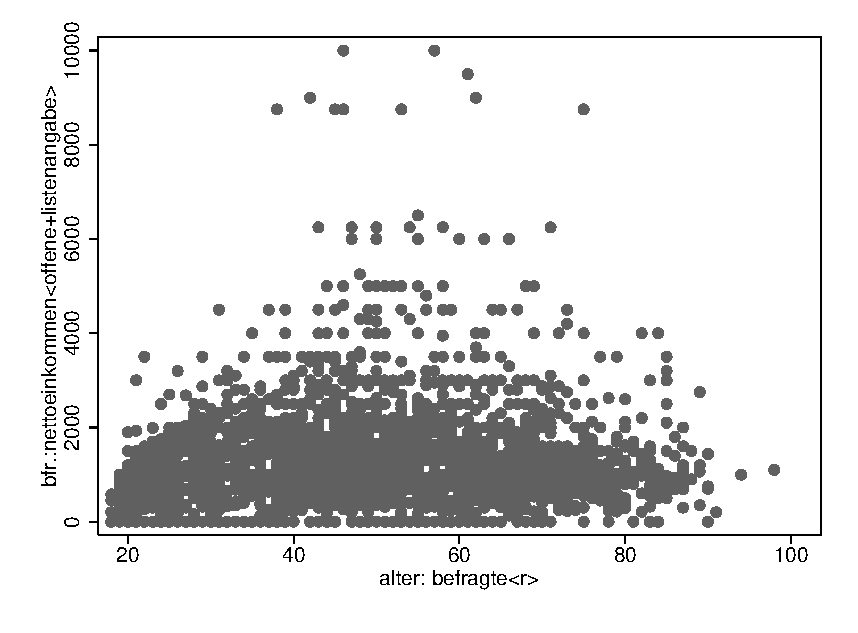
\includegraphics[width=8cm]{images/scatter.eps}}
\end{figure}
\end{frame}

\section{Boxplots}
\begin{frame}[fragile]{Boxplots} \index{Graphics!Boxplots} \index{Graphics!graph box}
\begin{lstlisting}
graph box weight
\end{lstlisting}
\begin{figure}
{\centering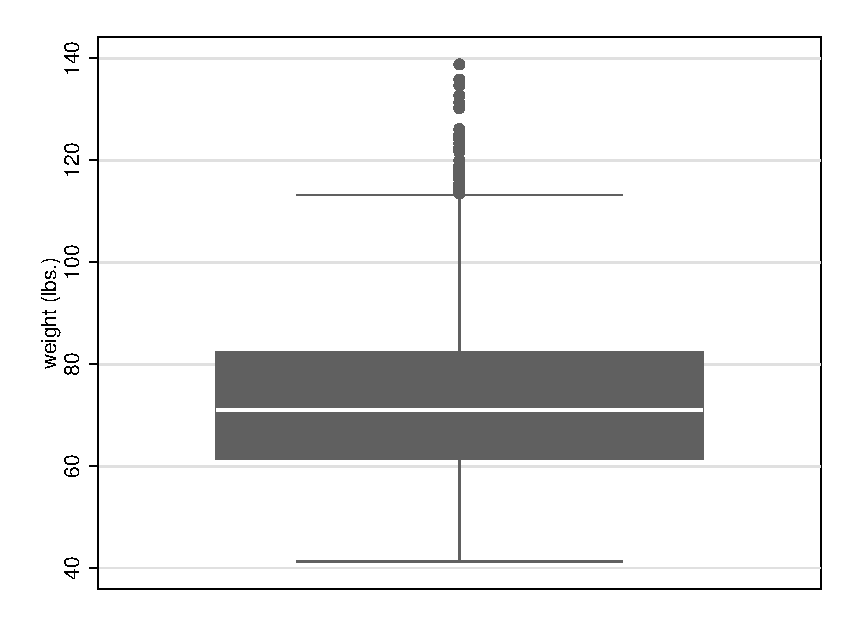
\includegraphics[width=8cm]{images/box.eps}}
\end{figure}
\end{frame}

\section{Histograms}
\begin{frame}[fragile]{Histograms} \index{Graphics!Histograms} \index{Graphics!hist} \index{Graphics!hist freq}
\begin{lstlisting}
hist weight, freq
\end{lstlisting}
\begin{figure}
{\centering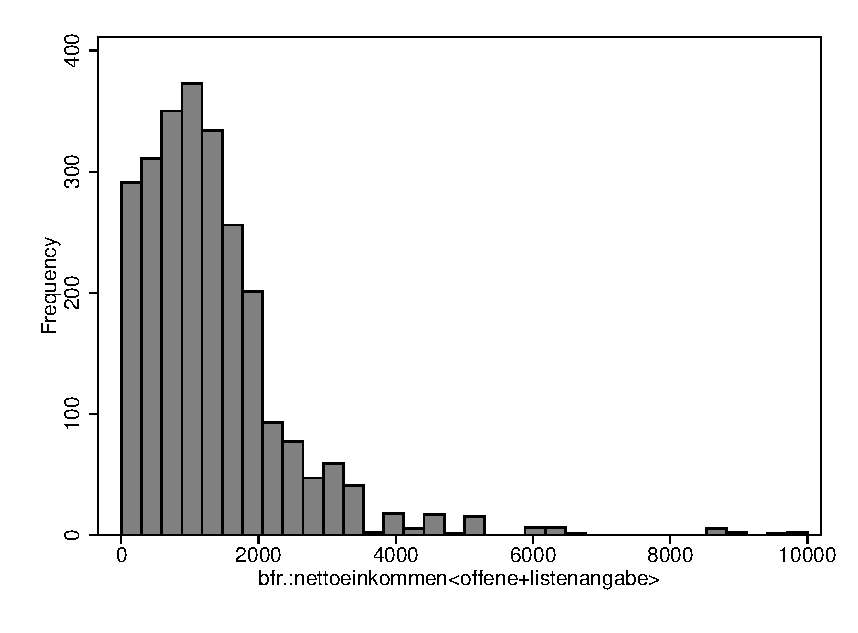
\includegraphics[width=8cm]{images/hist.eps}}
\end{figure}

  \begin{tikzpicture}[transform shape, rotate=10, overlay]
\node at (8,2) [mybox] (box) {%
    \begin{minipage}[t!]{0.35\textwidth}
    \tiny\textcolor{black}{\texttt{freq creates frequencies, else the y axis will show density.}}
    \end{minipage}
    };
\end{tikzpicture}

\end{frame}

\section{Dot-Charts}
\begin{frame}[fragile]{Dot-Charts} \index{Graphics!Dot-Charts} \index{Graphics!graph dot} \index{Graphics! graph dot over()}
\begin{lstlisting}
graph dot (mean) weight, over(sex)
\end{lstlisting}
\begin{figure}
{\centering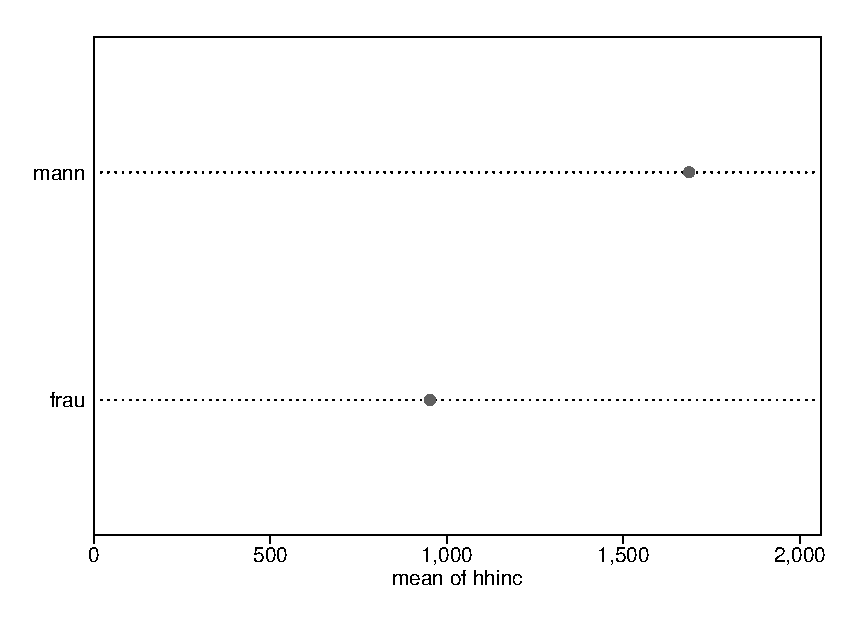
\includegraphics[width=8cm]{images/dot.eps}}
\end{figure}
\end{frame}


\section{Export of Graphics}
\begin{frame}[fragile]{Export of Graphics} \index{Graphics!export}
\begin{lstlisting}
graph export "D:/Data/graphics/graph1.pdf", replace
\end{lstlisting}
\begin{itemize}
\item For export there are many different formats
\item .ps .pes .wmf .emf .pdf .png .tif
\item For usage in MS-Office a good choice is .png
\item For usage in TeX a good choice is either .pdf or .eps
\end{itemize}
\end{frame}